\def\tutdate{18.11.2019}

\documentclass[handout]{beamer}
\usepackage{../templates/beamerthemekit}
%\usepackage[T1]{fontenc}

\usepackage[utf8]{inputenc}
\usepackage[T1]{fontenc}
\usepackage[ngerman]{babel}
\usepackage{listings}
\usepackage{hyperref}
\usepackage{graphicx}

\usepackage{amsmath}
\usepackage{amsthm}
\usepackage{amssymb}
\usepackage{polynom}

%\usepackage{ifthen}
%\usepackage{adjustbox} % for \adjincludegraphics

%\usepackage{tikz}
\usepackage{listings}

%\usepackage[]{algorithm2e}

%\usepackage{colortbl}
\usepackage{verbatim}
%\usepackage{alltt}
%\usepackage{changes}

%\usepackage{pdfpages}
%\usepackage{tabularx}

%\usepackage{euler}


\newcommand{\markBlue}[1]{\textcolor{kit-blue100}{#1}}
\newcommand{\markGreen}[1]{\textcolor{kit-green100}{#1}}
\newcommand{\vertspace}{\vspace{.2cm}}

%\newcommand{\#}{\markBlue{#1}}

%\newcommand{\pitem}{\pause\item}
\newcommand{\p}{\pause}

% -- MATH MACROS
\newcommand{\thistheoremname}{}
\newcommand{\G}{\mathbb{Z}}
\newcommand{\B}{\mathbb{B}}
\newcommand{\R}{\mathbb{R}}
\newcommand{\N}{\mathbb{N}}
\newcommand{\Q}{\mathbb{Q}}
\newcommand{\C}{\mathbb{C}}
\newcommand{\Z}{\mathbb{Z}}
\newcommand{\F}{\mathbb{F}}
\newcommand{\mi}{\mathrm{i}}
\renewcommand{\epsilon}{\varepsilon}
\newcommand{\okalk}{\mathscr{O}}


\newenvironment<>{taskblock}[1]{%
	\setbeamercolor{block title}{fg=kit-orange15,bg=kit-orange100}
	\setbeamercolor{block body}{fg=black,bg=kit-orange30}%
	\begin{block}#2{#1}}{\end{block}}

\setbeamertemplate{enumerate items}[default]

% Aussagenlogik Symbole
\newcommand{\W}{w}
\renewcommand{\F}{f}

% Kodierung
\newcommand{\frepr}{\textbf{repr}}
\newcommand{\fRepr}{\textbf{Repr}}
\newcommand{\fZkpl}{\textbf{Zkpl}}
\newcommand{\fbin}{\textbf{bin}}
\newcommand{\fdiv}{\textbf{ div }}
\newcommand{\fmod}{\textbf{ mod }}

% Speicherabbild
\newenvironment{memory}{\begin{tabular}{r | l}Adresse&Wert\\\hline\hline}{\end{tabular}}
\newcommand{\memrow}[2]{#1 & #2 \\\hline}

% Praedikatenlogik
\newcommand{\objequiv}{\stackrel{\cdot}{=}}
\newcommand{\pval}{val_{D,I,\beta}}

% Neue Befehle
\newcommand{\ip}{\pause} % inline pause, für mitten im satz
\newcommand{\pitem}{\pause\item} % für aufzählungen
\newcommand{\bp}{\pause} % block pause, für zwischen blöcken
\title[Grundbegriffe der Informatik]{ICPC\\Gruppe 2}
\date{\tutdate}
\subtitle{\tutTitle}
\author{Elias Schaut, Dennis Kobert, Niklas Kniep, Lam Vo, Ilia Bozhinov}

\institute{}

\titleimage{bg}
%\titleimage{bg-advent}

%
\ifthenelse{\equal{\compiletype}{livebeamer}}
	{
		\def\livebeamermode{1}
	}{}

\ifthenelse{\equal{\compiletype}{print}}
	{
		\def\printmode{1}
	}{}

\setbeamercovered{invisible}

%\usepackage[citestyle=authoryear,bibstyle=numeric,hyperref,backend=biber]{biblatex}
%\addbibresource{templates/example.bib}
%\bibhang1em

	
\def\tutTitle{Übersetzungen/Kodierungen, Zweierkomplement, Huffman-Codierung}
\begin{document}

\selectlanguage{ngerman}

%title page
\begin{frame}
	\titlepage
\end{frame}

\section{Hinweise}

\begin{frame} {Häufige Fehler}
	\begin{itemize}
		\item Wahrheitstabellen beginnen mit fff und \grqq zählen\grqq{}  dann hoch 
		\item fff, ffw, fwf, fww, wff, wfw, wwf, www (wie Binärzahlen)
		\pitem $B_1 \equiv B_2$ um zu zeigen, dass zwei Ausdrücke für jede Belegung gleichen Wahrheitswert haben
		\item $(a \land b) \lor b \equiv b$
		\pitem $f:\N_0 \times \N_0\rightarrow \N_0$ Zeige etwas für alle $n \in \N_0$
		\item $f(n+1, n+1) =  2f(n, n) + f(n + 1, n - 1) + f(n - 1, n + 1)$
		\item Wie muss Induktionsanfang/voraussetzung lauten?
		\pitem IA für $n = 0$ und $n = 1$
		\pitem IV: Behauptung gelte für ein $n \in N_+$
	\end{itemize}
\end{frame}


\section{Übersetzung und Kodierung}

\begin{frame}{Herführung zu Zahlendarstellungen}
	\pause Wir betrachten die Alphabete $A_{dez} := \Z_{10}, A_{bin} := \{0, 1\}, A_{oct} := \Z_8$.
	\begin{itemize}
		\pitem Was können wir daraus machen?
		\pitem $A_{dez}^* \supset \{42, 1337, 999\}$.
		\pitem $A_{bin}^* \supset \{101010, 10100111001, 1111100111\}$.
		\pitem $A_{oct}^* \supset \{52, 2471, 1747\}$.
		\pitem Wir suchen eine Möglichkeit, diese \markGreen{Zahlen} zu \markGreen{deuten}.
		\pitem Aber irgendwie so, dass $42_{\in A_{dez}} \stackrel{Deutung}{=} 101010_{\in A_{bin}} \stackrel{Deutung}{=} 52_{\in A_{oct}}$.
	\end{itemize}
\end{frame}

\subsection{Kodierung von Zahlen}

\begin{frame}{Definition von Zahlendarstellungen}
	\pause
	
	\begin{block}{$Num_k$}
		Einer Zeichenkette $Z_k$ aus Ziffern \p wird mit $Num_k$ eine eindeutige Zahl zugeordnet:
		
		\vspace{.2cm}
		
		\vspace{.2cm}
		
		 \p $Num_k(\epsilon) = 0$
		
		\vspace{.2cm}
		
		 \p $Num_k(wx) = k \cdot Num_k(w) + num_k(x)$ mit $w \in Z_k^*$ und $x \in Z_k$.
	\end{block}

	\pause
	
	\begin{block}{$num_k$}
		Einer einzelnen Ziffer $x \in Z_k$ aus einem Alphabet von Ziffern $Z_k$ wird mit $num_k(x)$ der Wert der Zahl zugewiesen.
	\end{block}

	\pause
	
	\begin{itemize}
		\item Wichtig: $Num_k(w) \neq num_k(w)$!
		\pitem Was ist: $num_{10}(3) \p = 3\p , num_{10}(7) \p = 7\p , num_{10}(11) = \p $ nicht definiert.
		\pitem Für Zahlen $\geq k$: Benutze $Num_k$!
	\end{itemize}
\end{frame}

\begin{frame}{Beispiel zu Zahlendarstellungen}
	$Num_k(\epsilon) = 0$.
	
	$Num_k(wx) = k \cdot Num_k(w) + num_k(x)$ mit $w \in Z_k^*$ und $x \in Z_k$.
	
	\vspace{.3cm}
	
	\p Was ist $Num_{10}(123)$?
	\begin{itemize}
		\pitem $Num_{10}(123) \p = 10 \cdot Num_{10} (12) + num_{10}(3) \p = 10 \cdot ( Num_{10} (1) + num_{10}(2)) + num_{10}(3) \p = 10 \cdot ( num_{10}(1) + 10 \cdot num_{10}(2) ) + num_{10}(3) \p = 10 \cdot 10 \cdot 1 + 10 \cdot 2  + 3 \p = 123$.
	\end{itemize}
	\p Yay?
	
	\p Was ist der dezimale Zahlenwert der Binärzahl 1010? \p Diesmal Basis $k = 2$.
	\begin{itemize}
		\pitem $Num_{2}(1010) \p = 2 \cdot Num_2(101) + num_2(0) \p = 2 \cdot (2 \cdot Num_2(10) + num_2(1) + num_2(0) \p = 2 \cdot (2 \cdot (2 \cdot Num_2(1) + num_2(0) ) + num_2(1) ) + num_2(0) \p = 2 \cdot (2 \cdot (2 \cdot num_2(1) + num_2(0) ) + num_2(1) ) + num_2(0) \p = 2 \cdot ( 2 \cdot (2 \cdot 1 + 0) + 1) + 0) = 10$.
	\end{itemize}
	\p Yay!
\end{frame}

\begin{frame}{Aufgaben zu Zahlendarstellungen}
	$Num_k(\epsilon) = 0$.
	
	$Num_k(wx) = k \cdot Num_k(w) + num_k(x)$ mit $w \in Z_k^*$ und $x \in Z_k$.
	
	\begin{taskblock}{Übungen zu Zahlendarstellungen}
		Berechne den numerischen Wert der folgenden Zahlen anderer Zahlensysteme nach dem vorgestellten Schema:
		\begin{itemize}
			\item $Num_8(345)$.
			\item $Num_2(11001)$.
			\item $Num_2(1000)$.
			\item $Num_4(123)$.
			\item $Num_{16}(4DF)$. (Zusatz)
		\end{itemize}
	\end{taskblock}

	Anmerkung: Hexadezimalzahlen sind zur Basis $16$ und verwenden als Ziffern (in aufsteigender Reihenfolge: $1, 2, 3, 4, 5, 6, 7, 8, 9, A, B, C, D, E, F$.
\end{frame}

\begin{frame}{Aufgaben zu Zahlendarstellungen}
	\pause Lösungen:
	\begin{itemize}
		\pitem $Num_8(345) \p = 229$.
		\pitem $Num_2(11001) \p = 25$.
		\pitem $Num_2(1000) \p = 8$.
		\pitem $Num_4(123) \p = 27$.
		\pitem $Num_{16}(4DF) \p = 1247$. 
	\end{itemize}
\end{frame}

\begin{frame}{Einfachere Umrechnung von Zahlendarstellungen}
	Es gilt: $2(2(2(2(2 \cdot 1 + 0)+1)+0)+1)+0 \p = 2^5 \cdot 1 + 2^4 \cdot 0 + 2^3 \cdot 1 + 2^2 \cdot 0 + 2^1 \cdot 1 + 2^0 \cdot 0$.
	
	\p Daher, einfachere Rechenweise: $Num_k(w) = k^0 \cdot w(0) + k^1 \cdot w(1) + k^2 \cdot w(2) + ...$.
	
	\p Was sind folgende Zahlen in Dezimal im Kopf gerechnet?
	
	\begin{itemize}
		\pitem $Num_2(10101) \p = 21$.
		\pitem $Num_2(11101) \p = 29$.
		\pitem $Num_2(1111111111) \p = 1023$.
	\end{itemize}
	
\end{frame}
		
\begin{frame}{Einfachere Umrechnung von Zahlendarstellungen}
	$Num_k(w) = k^0 \cdot w(0) + k^1 \cdot w(1) + k^2 \cdot w(2) + ...$.
	
	\p Was sind folgende Zahlen in Dezimal im Kopf gerechnet?
	
	\begin{itemize}
		\pitem $Num_{16}(A1) \p = 161$.
		\pitem $Num_{16}(BC) \p = 188$.
		\pitem $Num_{16}(14) \p = 20$.
	\end{itemize}
	
\end{frame}
\begin{frame}
\begin{itemize}
	\pitem Ist Num injektiv? \pause $Num_2(01) = Num_2(1)$
	\pitem Ist Num surjektiv? \pause Ja
\end{itemize}
\end{frame}

\begin{frame}{Rechnen mit $div$ und $mod$}
\pause
\begin{block}{$div$ Funktion}
	Die Funktion $div$ \markGreen{dividiert ganzzahlig.} \p (Schneidet also den Rest ab).
\end{block}
\pause
\begin{block}{$mod$ Funktion}
	Die Modulo Funktion $mod$ gibt den \markGreen{Rest einer ganzzahligen Division} zurück.
\end{block}
\pause
\begin{itemize}
	\item $22$ div $8 \p = 2 \p $ $(\frac{22}{8} = 2,75)$.
	\pitem $22$ mod $8 \p = 6$.
\end{itemize}

\pause Fülle die Tabelle aus:

\begin{tabular}{r | c c c c c c c c c c c c c}
	x & 0 & 1 & 2 & 3 & 4 & 5 & 6 & 7 & 8 & 9 & 10 & 11 & 12\\\hline
	x $div$ 4 & \p 0 & \p 0 & \p 0 & \p 0 & \p 1 & \p 1 & \p 1 & \p 1 & \p 2 & \p 2 & \p 2 & \p 2& \p 3\\
	x $mod$ 4 & \p 0 & \p 1 & \p 2 & \p 3 & \p 0 & \p 1 & \p 2 & \p 3 & \p 0 & \p 1 & \p 2 & \p 3& \p 0\\
\end{tabular}
\end{frame}

\subsection{Repräsentation von Zahlen}

\newcommand{\definitionOfRepr}{
\begin{align*}
\fRepr_k(n) =
\begin{cases}
\frepr_k(n) & \text{ falls } n < k \\
\fRepr_k(n \text{ div } k) \cdot \frepr_k(n \text{ mod } k) & \text{ falls } n \geq k
\end{cases}
\end{align*}
}

\begin{frame}{Von Zeichen zu Zahlen zurück zu Zahlen}
$11101_2$ ist also $29_{10}$. \p Was ist $29_{10}$ in binär? \pause
\begin{block}{$k$-äre Darstellung}
Die Repräsentation einer Zahl $n$ \p zur Basis $k$ \p lässt sich wie folgt ermitteln:\p
\definitionOfRepr
\p Achtung! \p Das $\cdot$ Symbol steht für Konkatenation, nicht für Multiplikation!
\end{block}
\end{frame}

\begin{frame}{Beispiel zu $Repr_k$}
\definitionOfRepr

\pause Zum Beispiel: \p 
\begin{align*}
\fRepr_2(29) 
\only<+->{&= \fRepr_2(29 \fdiv 2) \cdot \frepr_2(29 \fmod 2)}  \\
\only<+->{&= \fRepr_2(14) \cdot \frepr_2(1) \\}
\only<+->{&= \fRepr_2(14 \fdiv 2) \cdot \frepr_2(14 \fmod 2) \cdot 1} \\
\only<+->{&= \fRepr_2(7) \cdot \frepr_2(0) \cdot 1 }\\
\only<+->{&= \fRepr_2(7 \fdiv 2) \cdot \frepr_2(7 \fmod 2) \cdot 01} \\
\only<+->{&= \fRepr_2(3) \cdot \frepr(1) \cdot 01 }\\
\only<+->{&= \fRepr_2(3 \fdiv 2) \cdot \frepr(3 \fmod 2) \cdot 101} \\
\only<+->{&= \fRepr_2(1) \cdot \frepr(1) \cdot 101} \\
\only<+->{&= 11101}
\end{align*}
\end{frame}
\newcommand{\uhd}{_{16}}

\begin{frame}{Beispiel zu $Repr_k$}
\definitionOfRepr

\pause Beispiel mit Hexadezimalzahlen: \p 
\begin{align*}
\fRepr\uhd (29) 
\only<+->{&= \fRepr\uhd (29 \fdiv 16) \cdot \frepr\uhd (29 \fmod 16)}  \\
\only<+->{&= \fRepr\uhd (1) \cdot \frepr\uhd (13)}\\
\only<+->{&= 1 \cdot D = 1D}
\end{align*}
\end{frame}

\begin{frame}{Übung zu $Repr_k$}
\definitionOfRepr
\begin{taskblock}{Übung zu $Repr_k$}
Berechne die Repräsentationen folgender Zahlen in gegebenen Zahlensystemen:
\begin{itemize}
\item $\fRepr_2(13)$.
\item $\fRepr_4(15)$.
\item $\fRepr\uhd (268)$.
\end{itemize}
\end{taskblock}

\begin{itemize}
\pitem $\fRepr_2(13) \p = 1101$.
\pitem $\fRepr_4(15) \p = 33$.
\pitem $\fRepr\uhd (268) \p = 10C$.
\end{itemize}
\end{frame}

\subsection{Zweierkomplement-Darstellung}

\begin{frame}{Feste Länge von Binärzahlen}
\pause

\begin{block}{$bin_\ell$}
Die Funktion $\fbin_{\ell}\colon \Z_{2^{\ell}} \to \{0,1\}^{\ell}$ \p  bringt eine gegebene Binärzahl auf eine feste Länge\p , indem sie mit Nullen vorne aufgefüllt wird. \p Formell wird sie definiert als:\p
\begin{align*}\fbin_{\ell}(n) = 0^{\ell- |\fRepr_2(n)|} \fRepr_2(n)\end{align*}
\end{block}

\pause Beispiel:
\begin{itemize}
\pitem $\fbin_8(3) \p = 0^{8 - |\fRepr_2(3)|}\fRepr_2(3) \p = 0^{8 - |11|}\cdot 11 \p = 0^{8 - 2} \cdot 11 \p = 0^6 \cdot 11 = 00000011$.
\pitem $\fbin_{16}(3) \p = 0000000000000011$.
\end{itemize}
\end{frame}

\newcommand{\definitionOfZkpl}{
\begin{align*}
\fZkpl_{\ell}(x) =
\begin{cases}
0 \fbin_{\ell-1}(x) & \text{ falls } x\geq 0 \\
1 \fbin_{\ell-1}(2^{\ell-1} + x) & \text{ falls } x< 0 
\end{cases}
\end{align*}
}

\begin{frame}{Zweierkomplement}
\p Was ist mit negative Zahlen?

\begin{itemize}
\pitem Idee: Verwende das erste Bit, um zu speichern, ob die Zahl positiv oder negativ ist.
\pitem Beispiel: \p $5 = \markGreen{0}101_{zkpl}$\p , $-5 = \markGreen{1}011_{zkpl}$.
\end{itemize}

\pause

\begin{block}{Zweierkomplement Darstellung}
Die Zweierkomplementdarstellung einer Zahl $x$ \p mit der Länge $\ell$ ist wie folgt definiert:\p
\definitionOfZkpl		
\end{block}

\begin{itemize}
\pitem Wieso $\ell - 1$?
\end{itemize}

\end{frame}

\begin{frame}{Aufgaben zu Zweierkomplement-Darstellung}
\definitionOfZkpl

Was sind folgende Zahlen in Zweierkomplement-Darstellung?
\begin{itemize}
\item $\fZkpl_4 (3)$ \visible<1>{$=0011$.}
\item $\fZkpl_4 (7)$ \visible<2>{$=0111$.}
\item $\fZkpl_4 (-5)$ \visible<3>{$=1011$.}
\item $\fZkpl_8 (13)$ \visible<4>{$=0000 1101$.}
\item $\fZkpl_8 (-34)$ \visible<5>{$=1101 1110$.}
\item $\fZkpl_8 (-9)$ \visible<6>{$=1111 0111$.}
\end{itemize}
\end{frame}

\begin{frame} {Übersetzungen}
\begin{block} {Definition der Semantikabbildung}
Sei \textit{Sem} die Menge der Bedeutungen. \p Ferner seien $A$ und $B$ Alphabete \p und $L_A \subseteq A^* \text{ und } L_B \subseteq B^*$.\\
\p Weiter sei $sem_A:L_A \rightarrow Sem$ \p und $sem_B: L_B \rightarrow Sem$\\
\p Dann heißt $f: L_A \rightarrow L_B$ Übersetzung \p , wenn gilt: für jedes $w \in L_A$ gilt $sem_A(w) = sem_B(f(w))$.
\end{block}
\begin{itemize}
\pitem Bedeutungserhaltende Abbildungen von Wörtern auf Wörter
\end{itemize}
\textbf{Beispiel}\\
\p Betrachte $Trans_{2,16}: \mathbb{Z}_{16}^* \rightarrow \mathbb{Z}_{2}^*$ mit $ Trans_{2,16}(w) = Repr_2(Num_{16}(w))$
\begin{itemize}
\pitem $Trans_{2,16}(A3) = Repr_2(Num_{16}(A3)) = Repr_2(163) = 10100011$
\end{itemize}
\end{frame}
\begin{frame}{Wozu Übersetzungen}
\begin{itemize}
\pitem Lesbarkeit (vergleiche $DF_{16}$ mit $11011111_2$)
\pitem Verschlüsselung
\pitem Kompression (Informationen platzsparend aufschreiben)
\pitem Kontextabhängige Semantiken (Deutsch $\rightarrow$ Englisch)
\pitem Fehlererkennung
\end{itemize} 
\end{frame}


\begin{frame}{Codierungen}	
\begin{block}{Definitionen}
\begin{itemize}
\pitem Codewort $f(w)$ \p einer Codierung $f: L_A \rightarrow L_B$
\pitem Code: $\{f(w)|w \in L_A\} = f(L_A)$
\pitem Codierung: \textbf{Injektive} Übersetzung
\begin{itemize}
\pitem Ich komme immer eindeutig von einem Codewort f(w) zu $w$ zurück
\end{itemize}
\end{itemize}
\end{block}\p
\textbf{Bemerkung}\\
\begin{itemize}
\pitem Was ist, wenn $L_A$ unendlich ist (man kann nicht alle Möglichkeiten aufzählen)
\pitem Auswege: Homomorphismen, Block-Codierungen
\end{itemize}
\end{frame}


\subsection{Homomorphismen}

\begin{frame}{Homomorphismen}
\begin{block} {Definition von Homomorphismen}\p
Seien $A, B$ Alphabete. \p Dann ist $h: A^* \rightarrow B^*$ \p ein Homomorphismus\p , falls für alle $w_1, w_2 \in A^*$ gilt:\\ \p
\begin{equation*}
h(w_1w_2) = h(w_1)h(w_2)
\end{equation*}
\end{block}

\begin{itemize}
\pitem Ein Homomorphismus ist Abbildung, die mit Konkatenation verträglich ist
\pitem Homomorphismus ist $\varepsilon$-frei, wenn für jedes $x \in A: h(x) \neq \varepsilon$
\pitem Homomorphismen lassen das leere Wort unverändert, also $h(\varepsilon) = \varepsilon$
\end{itemize}
\end{frame}

\begin{frame}
Sei $h$ ein Homomorphismus.

\begin{taskblock}{Übung zu Homomorphismen}
\begin{enumerate}
\pitem $h(a) = 001$ und $h(b) = 1101$. Was ist dann $h(bba)$? 
\pitem[$\rightarrow$] $h(bba) = h(b)h(b)h(a) = 1101 \cdot 1101 \cdot 001 = 11011101001$
\pitem Sei $h(a) = 01, h(b) = 11 \text{ und } h(c) = \varepsilon$. Nun sei $h(w)= 011101$. Was war $w$? 
\pitem[$\rightarrow$] $aba$ oder $cabccac$, ... Allgemein: $w \in \{c\}^* \cdot \{a\} \cdot \{c\}^* \cdot \{b\} \cdot \{c\}^* \cdot \{a\} \cdot \{c\}^*$ \\ \p $\epsilon$-Freiheit hat also die Eindeutigkeit zerstört!
\pitem Kann h aus 2 eine Codierung sein?
\pitem[$\rightarrow$] Nein, da nicht injektiv!
\pitem Warum will man $\varepsilon$-freie Homomorphismen?
\pitem[$\rightarrow$] Information geht sonst verloren!
\pitem Was heißt hier ``Information geht verloren''? 
\pitem[$\rightarrow$] Es gibt $w_1 \neq w_2$ mit $h(w_1) = h(w_2)$
\end{enumerate}
\end{taskblock}
\end{frame}

\begin{frame}
\begin{itemize}
\pitem Information kann auch anders ``verloren'' gehen
\pitem[$\rightarrow$] z.B. $h(a) = 0, h(b) = 1, h(c) = 10$ \p -- Wie das?
\end{itemize} \pause
\begin{block}{Präfixfreiheit}
\p Gegeben ist ein Homomorphismus $h: A^* \rightarrow B^*$.\\
\p Wenn für keine zwei verschiedenen $x_1, x_2 \in A$ gilt\p , dass $h(x_1)$  Präfix von $h(x_2)$ ist\p , dann ist $h$ präfixfrei. 
\end{block}
\pause
\begin{block}{Satz}
Präfixfreie Codes sind injektiv.
\end{block} \pause
\textbf{Beispiele}\\
\begin{itemize}
\pitem $h(a) = 01 \text{ und } h(b) = 1101 $ ist präfixfrei
\pitem $g(a) = 01 \text{ und } g(b) = 011$ ist nicht präfixfrei
\end{itemize}
\end{frame}

\subsection{Huffman Codierung}

\begin{frame}{Huffman-Codierung}
\begin{itemize}
\pitem Komprimiert eine Zeichenkette
\pitem Kodiert häufiger vorkommende Zeichen zu kürzeren Codewörter als Zeichen die seltener vorkommen.
\pitem Vorgehensweise:
\begin{enumerate}
\pitem Zähle Häufigkeiten aller Zeichen der Zeichenkette
\pitem Schreibe alle vorkommenden Zeichen und ihre Häufigkeiten nebeneinander
\pitem Wiederhole, bis der Baum fertig ist:
\begin{itemize}
\pitem Verbinde die zwei Zeichen mit niedrigsten Häufigkeiten zu neuem Knoten über diesen
\pitem Dieser hat als Zahl die aufsummierte Häufigkeiten
\end{itemize}
\pitem Danach: Alle linken Kanten werden mit $0$ kodiert, alle rechten Kanten mit $1$
\end{enumerate}
\end{itemize}

\p Das Ergebnis ist eine Zeichenkette aus $\{0,1\}$\p , die kürzer ist als die ursprüngliche Zeichenkette in binär.
\end{frame}

\begin{frame}{Huffman-Codierung}
Gegeben
\begin{itemize}
\item $w \in A^*$ 
\only<1>{ \\ }\textbf{w } = \texttt{ afebfecaffdeddccefbeff }
\pause
\item Anzahl der Vorkommen aller Zeichen in w ($N_x(w)$)
\end{itemize}		
\only<2>{
\textbf{Häufigkeiten:}\\
\begin{tabular}{c c c c c c c}
\hline
x &a&b&c&d&e&f\\
\hline
$N_x(w)$& 2& 2&3&3& 5& 7\\
\hline
\end{tabular}							
}
\pause
Zwei Phasen zur Bestimmung eines Huffman-Codes
\begin{enumerate}
\item Konstruieren eines ``Baumes''
\begin{itemize}
\item Blätter entsprechen den Zeichen
\item Kanten mit 0 und 1 beschriften\\ 
\only<3>{
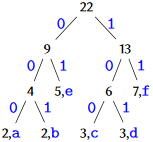
\includegraphics[scale=0.8]{../images/Baum.PNG}
\begin{tabular}{c c c c c c c}
\textbf{Häufigkeiten:}\\
\hline
x  &a&b&c&d&e&f\\
\hline
$N_x(w)$& 2& 2&3&3& 5& 7\\
\hline
\end{tabular}	
}
\end{itemize} 
\pause
\item Ablesen der Codes aus dem Baum (Pfadbeschriftungen)
\end{enumerate}
\only<4>{
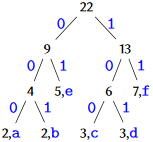
\includegraphics[scale=0.46]{../images/Baum.png}
\hspace{0.4cm}
\begin{tabular}{c c c c c c c}
\textbf{Häufigkeiten:}\\
\hline
x &a&b&c&d&e&f\\
\hline
$N_x(w)$ & 2& 2&3&3& 5& 7\\

\textbf{Codewörter:}\\
\hline
x &a&b&c&d&e&f\\
\hline
h(x)& 000& 001&100&101& 01& 11\\
\hline
\end{tabular}							
}		
\end{frame}

\begin{frame}{Übung zu Huffman Codierung}
\begin{taskblock}{Übung}
Sei $A = \{$\texttt a, b, c, d, e, f, g, h$\}$\\
\begin{itemize}
\item Codiere das Wort \texttt{badcfehg} mit Hilfe der Huffman-Codierung \pause
\item [$\rightarrow$]Mögliche Lösung: 001 100 010 011 101 000 111 110
\pause
\item Wie lauten die Codewörter, wenn für das Wort $w$ gilt: $N_a(w) = 1, N_b(w) = 2, N_c(w) = 2, N_d(w) =8, N_e(w) =16, N_f(w) =32, N_g(w) = 64, N_h(w) = 128$

\end{itemize} \pause
Mögliche Lösung:\\
\begin{tabular}{|c|c c c c c c c c|}
\hline
x &a&b&c&d&e&f&g&h\\
\hline
h(x)& 0000000& 0000001&000001&00001& 0001&001& 01&1\\
\hline
\end{tabular}
\end{taskblock}
\end{frame}	

\begin{frame}
\begin{itemize}
\item Wie lang wäre das zweite Wort (\texttt{abbcccc} $\texttt{d}^{8}$...$\texttt{g}^{64}\texttt{h}^{128}$) mit dem ersten Code codiert? 
\pause
\item[$\rightarrow$] 741 Symbole. Also dreimal so lang wie das Original. \pause
\item Wie lang wäre das zweite Wort mit dem zweiten Code codiert?\pause
\item[$\rightarrow$] 501 Symbole. Also nur zweimal so lang wie das Original. \pause
\item Was fällt euch auf?
\end{itemize}
\end{frame}		

\begin{frame}{Wahr oder falsch?}
Sei $h: A^* \rightarrow \mathbb{Z}_2$ eine Huffman-Codierung
\begin{itemize}
\item h ist ein $\varepsilon$-freier Homomorphismus \pause \textbf{Wahr!}\pause
\item Häufigere Symbole werden mit langen Worten codiert, seltene mit kürzeren \pause \textbf{Falsch!}\pause
\item Die Kompression ist am stärksten, wenn die Häufigkeiten aller Zeichen ungefähr gleich sind. \pause \textbf{Falsch!} \pause
\item h ist präfixfrei \pause \textbf{Wahr!} \pause
\item Es kann noch kürzere Codierungen geben \pause \textbf{Falsch!}
\end{itemize}
\end{frame}


\begin{frame}{Huffman-Codierung}
\begin{block}{Eigenschaften}
Sei $A$ ein Alphabet und $w \in A$. Dann gilt für die Huffman-Codierung h:
\begin{itemize}
\item $h: A^* \rightarrow \mathbb{Z}_2$
\item $h$ ist $\varepsilon$-freier Homomorphismus
\item $h$ ist präfixfreier Homomorphismus
\item Häufigere Symbole werden mit kurzen Worten codiert, seltene mit längeren
\item Produziert kürzestmögliche Codierungen
\end{itemize}
\end{block}
\end{frame}

\begin{frame}{Block-Codierung mit Huffman}
\begin{itemize}
\pitem Wir betrachten nicht mehr einzelne Symbole, sondern Blöcke von fester Länge $b > 1$
\pitem Blätter des Huffman-Baums sind jetzt \textit{Wörter der Länge b}
\end{itemize}

\vspace{.5cm}

Beispiel an der Tafel: Codierung von $aab\cdot deg \cdot deg \cdot aab \cdot ole \cdot aab \cdot deg \cdot aab$.\p

\vspace{.5cm}

\p
\begin{itemize}
\pitem Alphabet $A =\{$\texttt{a,b,c,d} $\}$
\pitem Text über $A$, der nur aus Teilwörtern der Länge 10 zusammengesetzt ist, in denen jeweils immer nur ein Symbol vorkommt
%\item z.B. \texttt{aaaaaaaaaabbbbbbbbbbcccccccccc}...
\pitem Angenommen $\texttt{a}^{10}$, ..., $\texttt{d}^{10}$ kommen alle gleich häufig vor. Wie lang ist dann die Huffman-Codierung? \pause
\pitem[$\rightarrow$] Ein Fünftel, weil jeder Zehnerblock durch zwei Bits codiert wird
\end{itemize}

\end{frame}

\begin{frame}{Wahr oder falsch?}
Sei $h: A^* \rightarrow \mathbb{Z}_2$ eine Huffman-Codierung
\begin{itemize}
	\item h ist ein $\varepsilon$-freier Homomorphismus \pause \textbf{Wahr!}\pause
	\item Häufigere Symbole werden mit langen Worten codiert, seltene mit kürzeren \pause \textbf{Falsch!}\pause
	\item Die Kompression ist am stärksten, wenn die Häufigkeiten aller Zeichen ungefähr gleich sind. \pause \textbf{Falsch!} \pause
	\item h ist präfixfrei \pause \textbf{Wahr!} \pause
	\item Es kann noch kürzere Codierungen geben \pause \textbf{Falsch!}
\end{itemize}
\end{frame}


\begin{frame}
	
\includegraphics[width=\linewidth]{../images/thatsall.png}
\end{frame}


\end{document}
